%-*-latex-*-
\sectionthree{Sparse matrix}
\begin{python0}
from solutions import *; clear()
\end{python0}

Here's a matrix:
\[
\begin{bmatrix}
1 & 3 & -1 & 2 \\
7 & 0 & 8 & 0 \\
8 & 0 & 9 & 2 \\
1 & 1 & 8 & 0 
\end{bmatrix}
\]
This is a rectangular array of numbers.
We can use a 2D array as a container for these values.

Suppose there are lots of zeroes in the matrix like this:
\[
\begin{bmatrix}
0 & 3 & 0 & 2 \\
0 & 0 & 0 & 0 \\
4 & 0 & 9 & 2 \\
1 & 1 & 8 & 0 
\end{bmatrix}
\]
Such a matrix is a \defone{sparse matrix}.
When the percentage of 0s is extremely high, instead of a 2D array,
one can use two arrays of doubly linked list like this:

\begin{center}
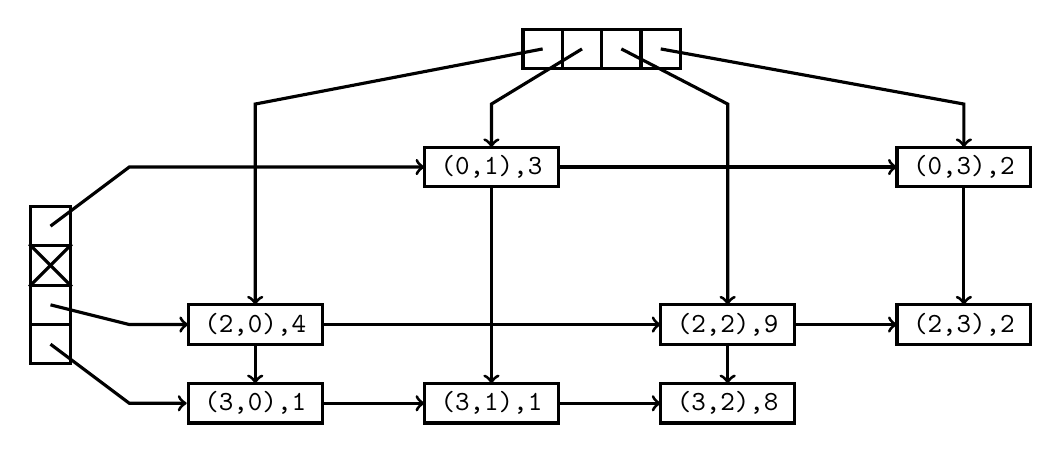
\begin{tikzpicture}

\draw (3.8499999999999996, 3.25)
  node[draw, line width=0.04cm, , color=black,
       rounded corners=0cm, inner sep=0cm] {

\begin{minipage}[t][0.5cm]{1.7cm}
\mbox{}

\end{minipage}

};\draw (3.8499999999999996, 3.25) node[color=black] {{\texttt{(0,1),3}}};
\draw (9.85, 3.25)
  node[draw, line width=0.04cm, , color=black,
       rounded corners=0cm, inner sep=0cm] {

\begin{minipage}[t][0.5cm]{1.7cm}
\mbox{}

\end{minipage}

};\draw (9.85, 3.25) node[color=black] {{\texttt{(0,3),2}}};
\draw (0.85, 1.25)
  node[draw, line width=0.04cm, , color=black,
       rounded corners=0cm, inner sep=0cm] {

\begin{minipage}[t][0.5cm]{1.7cm}
\mbox{}

\end{minipage}

};\draw (0.85, 1.25) node[color=black] {{\texttt{(2,0),4}}};
\draw (6.85, 1.25)
  node[draw, line width=0.04cm, , color=black,
       rounded corners=0cm, inner sep=0cm] {

\begin{minipage}[t][0.5cm]{1.7cm}
\mbox{}

\end{minipage}

};\draw (6.85, 1.25) node[color=black] {{\texttt{(2,2),9}}};
\draw (9.85, 1.25)
  node[draw, line width=0.04cm, , color=black,
       rounded corners=0cm, inner sep=0cm] {

\begin{minipage}[t][0.5cm]{1.7cm}
\mbox{}

\end{minipage}

};\draw (9.85, 1.25) node[color=black] {{\texttt{(2,3),2}}};
\draw (0.85, 0.25)
  node[draw, line width=0.04cm, , color=black,
       rounded corners=0cm, inner sep=0cm] {

\begin{minipage}[t][0.5cm]{1.7cm}
\mbox{}

\end{minipage}

};\draw (0.85, 0.25) node[color=black] {{\texttt{(3,0),1}}};
\draw (3.8499999999999996, 0.25)
  node[draw, line width=0.04cm, , color=black,
       rounded corners=0cm, inner sep=0cm] {

\begin{minipage}[t][0.5cm]{1.7cm}
\mbox{}

\end{minipage}

};\draw (3.8499999999999996, 0.25) node[color=black] {{\texttt{(3,1),1}}};
\draw (6.85, 0.25)
  node[draw, line width=0.04cm, , color=black,
       rounded corners=0cm, inner sep=0cm] {

\begin{minipage}[t][0.5cm]{1.7cm}
\mbox{}

\end{minipage}

};\draw (6.85, 0.25) node[color=black] {{\texttt{(3,2),8}}};\draw[line width=0.04cm,black,->] (4.7,3.25) to  (9,3.25);
\draw[line width=0.04cm,black,->] (7.7,1.25) to  (9,1.25);
\draw[line width=0.04cm,black,->] (1.7,0.25) to  (3,0.25);
\draw[line width=0.04cm,black,->] (4.7,0.25) to  (6,0.25);
\draw[line width=0.04cm,black,->] (3.85,3) to  (3.85,0.5);
\draw[line width=0.04cm,black,->] (6.85,1) to  (6.85,0.5);
\draw[line width=0.04cm,black,->] (9.85,3) to  (9.85,1.5);
\draw[line width=0.04cm,black,->] (1.7,1.25) to  (6,1.25);
\draw[line width=0.04cm,black,->] (0.85,1) to  (0.85,0.5);

\draw (-1.75, 2.5)
  node[draw, line width=0.04cm, , color=black,
       rounded corners=0cm, inner sep=0cm] {

\begin{minipage}[t][0.5cm]{0.5cm}
\mbox{}

\end{minipage}

};
\draw (-1.75, 2.0)
  node[draw, line width=0.04cm, , color=black,
       rounded corners=0cm, inner sep=0cm] {

\begin{minipage}[t][0.5cm]{0.5cm}
\mbox{}

\end{minipage}

};
\draw (-1.75, 1.5)
  node[draw, line width=0.04cm, , color=black,
       rounded corners=0cm, inner sep=0cm] {

\begin{minipage}[t][0.5cm]{0.5cm}
\mbox{}

\end{minipage}

};
\draw (-1.75, 1.0)
  node[draw, line width=0.04cm, , color=black,
       rounded corners=0cm, inner sep=0cm] {

\begin{minipage}[t][0.5cm]{0.5cm}
\mbox{}

\end{minipage}

};\draw[line width=0.04cm,black,->] (-1.75,2.5) to  (-0.75,3.25) to  (3,3.25);
\draw[line width=0.04cm,black] (-2.02,2.27) to  (-1.48,1.73);
\draw[line width=0.04cm,black] (-1.48,2.27) to  (-2.02,1.73);
\draw[line width=0.04cm,black,->] (-1.75,1.5) to  (-0.75,1.25) to  (0,1.25);
\draw[line width=0.04cm,black,->] (-1.75,1.0) to  (-0.75,0.25) to  (-0.02,0.25);

\draw (4.5, 4.75)
  node[draw, line width=0.04cm, , color=black,
       rounded corners=0cm, inner sep=0cm] {

\begin{minipage}[t][0.5cm]{0.5cm}
\mbox{}

\end{minipage}

};
\draw (5.0, 4.75)
  node[draw, line width=0.04cm, , color=black,
       rounded corners=0cm, inner sep=0cm] {

\begin{minipage}[t][0.5cm]{0.5cm}
\mbox{}

\end{minipage}

};
\draw (5.5, 4.75)
  node[draw, line width=0.04cm, , color=black,
       rounded corners=0cm, inner sep=0cm] {

\begin{minipage}[t][0.5cm]{0.5cm}
\mbox{}

\end{minipage}

};
\draw (6.0, 4.75)
  node[draw, line width=0.04cm, , color=black,
       rounded corners=0cm, inner sep=0cm] {

\begin{minipage}[t][0.5cm]{0.5cm}
\mbox{}

\end{minipage}

};\draw[line width=0.04cm,black,->] (4.5,4.75) to  (0.85,4.05) to  (0.85,1.5);
\draw[line width=0.04cm,black,->] (5.0,4.75) to  (3.85,4.05) to  (3.85,3.5);
\draw[line width=0.04cm,black,->] (5.5,4.75) to  (6.85,4.05) to  (6.85,1.5);
\draw[line width=0.04cm,black,->] (6.0,4.75) to  (9.85,4.05) to  (9.85,3.5);
\end{tikzpicture}

\end{center}



Note that each doubly linked node points to two nodes, the next node in the same row and
the next node in the same column.
Furthermore, each node appears twice, once in the array of linked list for rows
and once in the array of linked list for columns.

For instance look at the $(2,0)$ entry of the matrix. The value there is 4.
Therefore for this nonzero entry of the matrix,
we have a node with value \texttt{(2,0),4}.
Each node is in two linked list, a row listed list and a column linked list.
A row linked list links up nodes in the same row
and a column linked lists up nodes in the same column.
Clearly each node has two pointers, one pointing to the node
next in the row, and another pointing to the node next in the column.

Get it?

If a matrix is sparse, you can also use a hashtable -- I'll talk about
this later.
